% !TeX root = ../main.tex
% !TeX spellcheck = de_DE

{\bfseries\Huge\centering{
Grundlagen\\ 
\huge\itshape{
    Klasse E und A\\
    }
}}
\begin{figure}
    %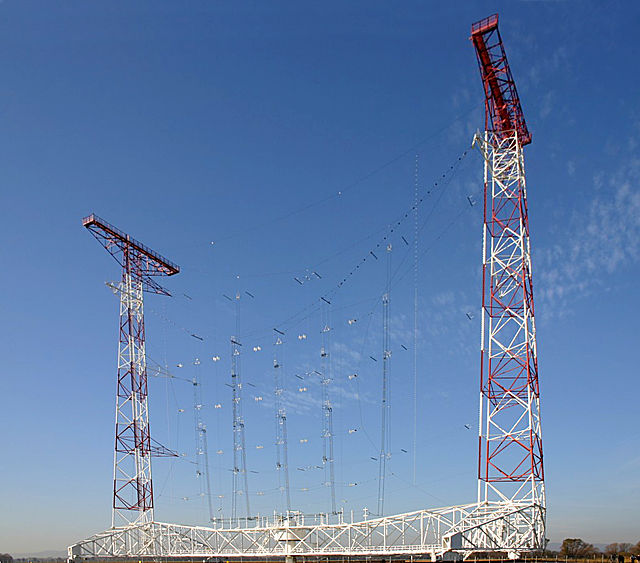
\includegraphics[]{assets/640px-Moosbrunn_SW_Antenna}
    %\caption{Kurzwellenstation Moosbrunn}  
\end{figure}        
\part[]{Zahlenwerte}
Wellenlänge $\lambda$ beschreibt den Abstand zwischen den Wellen.\newline
Die Frequenz beschreibt die Anzahl der Schwingungen. \newline
Die vereinfachte Formel zur Berechnung ist $ \frac{300}{MHz} $
Lichtgeschwindigkeit = 300.000km/sek \newline
\vskip0.4cm
Beispiel einer Wattrechnung mit Potenzen.\newline
\begin{math}
    750W = 750*10^0 \newline
    \hspace*{0.98cm} = 75 *10^1\newline
    \hspace*{0.98cm} = 7.5 * 10^2\newline
    \hspace*{0.98cm} = 0.75 * 10^3 \newline
\end{math}
\vskip0.4cm
Beispiel einer Umrechnung von verschiedenen Einheiten. \newline
\begin{math}
    1mm = 1*10^-3m = 1 \newline
    1\mu = 75 *10^1\newline
    1nn = 7.5 * 10^2\newline
    1pm = 0.75 * 10^3 \newline
\end{math}